% STASHED on 2026-05-31. This was the "Prediction heads" section at the end of
% Chapter 3 (Machine Learning). It is NOT \input anywhere, so it does not
% compile. The three heads are to be re-introduced in Chapter 4, alongside the
% models that use them, when we get to the analysis.
%
% UPDATE 2026-06-11: The von Mises--Fisher material below was folded into
% Chapter 4, \section{A learned per-event uncertainty as a final diagnostic}
% (label sec:vmf), in condensed form (density, NLL, sinh-overflow and
% unbounded-kappa notes). Do NOT re-introduce it again. The classification-head
% and direction-regression-head text is also covered inline in Chapter 4
% (sections sec:classifier and sec:direction_reco), so this file is now
% reference-only.

\section{Prediction heads}
\label{sec:prediction_heads}

The three branches at the bottom of Figure~\ref{fig:transformer_architecture} are, from left to right, a classification head, a direction-regression head, and a von Mises--Fisher head. The classification head asks whether an event is a stopped muon and returns that probability. The direction-regression head asks where the muon came from and returns a reconstructed arrival direction. The von Mises--Fisher head asks the same question but also how well that direction is pinned down, returning a direction together with a per-event uncertainty. The first drives the through-going/stopped split that opens the next chapter, and the other two carry the directional reconstruction that the later analysis relies on. Each is introduced in turn below, kept to what the head outputs and how it is trained, with the surrounding model-specific details left to the chapters where the models are built and used.

\subsection{Classification head}

The classification head maps the event vector to a single logit $\ell(\mathcal{E})$ through a small feed-forward network, and the probability that the event is a stopped muon follows from the sigmoid,
\[
    s(\mathcal{E}) = P(\mathrm{stopped}\mid\mathcal{E}) = \sigma\bigl(\ell(\mathcal{E})\bigr).
\]
This is the head used by the through-going/stopped classifier. That model wraps the head in two further ingredients, a set of event-level aggregates fused with the transformer output and a class-weighted training loss, so the full construction is laid out where the classifier is built in Section~\ref{sec:classifier} rather than repeated here. At the level of the architecture the head itself is just the sigmoid readout above.

\subsection{Direction-regression head}

The direction-regression head reads the same event vector and maps it to three numbers that are $L_2$-normalised onto the unit sphere, giving a predicted arrival direction $\hat{\mathbf{n}}\in S^2$. The network is trained on the opening angle $\Delta\Psi$ between the predicted and the true direction $\mathbf{n}$,
\[
    \cos\Delta\Psi = \hat{\mathbf{n}}\cdot\mathbf{n},
\]
so that minimising $\Delta\Psi$, equivalently maximising $\hat{\mathbf{n}}\cdot\mathbf{n}$, pulls the prediction toward the truth.

\subsection{von Mises--Fisher head}
\label{sec:vmf_method}

The direction-regression head just described hands back a single unit vector
$\hat{\mathbf{n}}$ per event. This is enough to estimate \emph{where} an event
came from, but it says nothing about \emph{how well} that estimate is
constrained. A long, brightly illuminated
through-going track and a short, sparse stopped event are handed back with the
same kind of answer, a bare direction, even though the detector plainly
determines one far better than the other. We will later want the network to
report not just a direction but its own confidence in that direction.

The natural way to do this is to let the model predict a probability
distribution \emph{on} the sphere rather than a point on it. The standard choice
for directional data is the von Mises--Fisher (vMF) distribution, the spherical
analogue of an isotropic Gaussian.
For a unit vector $\mathbf{x}\in S^{p-1}$ it reads
\[
    f_p(\mathbf{x};\boldsymbol\mu,\kappa)
    = C_p(\kappa)\,\exp\!\bigl(\kappa\,\boldsymbol\mu^\top\mathbf{x}\bigr),
    \qquad
    \boldsymbol\mu\in S^{p-1},\quad \kappa\ge 0,
\]
where $\boldsymbol\mu$ is the mean direction and $\kappa$ the concentration. For
directions in three dimensions, $p=3$, the normalisation takes the closed form
\[
    C_3(\kappa) = \frac{\kappa}{4\pi\sinh\kappa},
    \qquad\text{so}\qquad
    f_3(\mathbf{x};\boldsymbol\mu,\kappa)
    = \frac{\kappa}{4\pi\sinh\kappa}\,
      \exp\!\bigl(\kappa\,\boldsymbol\mu^\top\mathbf{x}\bigr).
\]
The density depends on the data only through
$\boldsymbol\mu^\top\mathbf{x}=\cos\Delta\Psi$, the cosine of the opening angle
to the mean direction, so it is rotationally symmetric about $\boldsymbol\mu$.
The single parameter $\kappa$ sets how tightly the distribution clusters around
$\boldsymbol\mu$: at $\kappa=0$ it is uniform over the sphere, and as $\kappa$
grows it concentrates into an ever-narrower cap. In the concentrated limit it
approaches a Gaussian in the tangent plane with angular spread
\[
    \sigma_\Psi \approx \frac{1}{\sqrt{\kappa}},
\]
so $\kappa$ plays the role of an inverse variance. A large $\kappa$ marks a
confident, well-constrained event and a small $\kappa$ an uncertain one.
Figure~\ref{fig:vmf_sphere} illustrates this for three values of $\kappa$.

\begin{figure}[H]
    \centering
    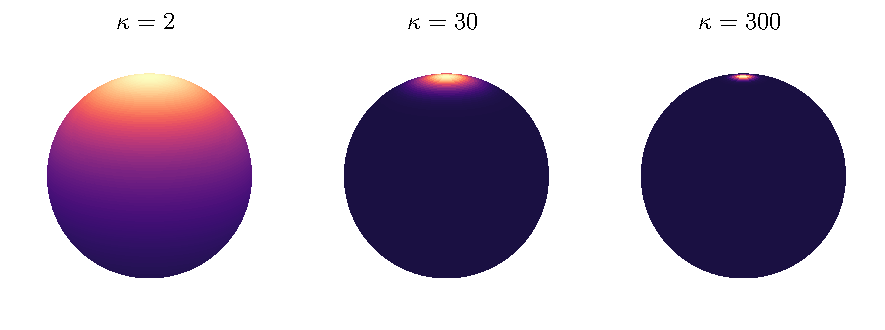
\includegraphics{figures/vmf_sphere.pdf}
    \caption{The von Mises--Fisher distribution on the sphere for three values of the concentration $\kappa$, with the mean direction $\boldsymbol\mu$ at the top. A small $\kappa$ spreads probability over a wide cap (an uncertain event). A large $\kappa$ concentrates it into a narrow one (a well-constrained event), with angular spread $\sigma_\Psi\approx1/\sqrt{\kappa}$.}
    \label{fig:vmf_sphere}
\end{figure}s

sConcretely, the directional head is replaced by one that emits four numbers per
event. Three are $L_2$-normalised into the mean direction $\boldsymbol\mu\in S^2$
exactly as before; the fourth is mapped to a positive concentration $\kappa$.
The model is then trained by maximum likelihood, i.e.\ by minimising the
negative log-likelihood of the true direction $\mathbf{n}$ under the predicted
distribution,
\[
    \mathcal{L}_{\mathrm{vMF}}
    = -\log f_3(\mathbf{n};\boldsymbol\mu,\kappa)
    = -\log\kappa + \log\sinh\kappa + \log(4\pi)
      - \kappa\,\boldsymbol\mu^\top\mathbf{n}.
\]
The last term still rewards aligning $\boldsymbol\mu$ with the truth, so the
point direction is learned for essentially the same reason as under the
opening-angle loss; the new ingredient is that the same objective also forces
$\kappa$ to be large only when that alignment is reliably good and small when it
is not. The model is penalised both for being wrong and for being overconfident,
and the value of $\kappa$ it settles on is a genuine, learned per-event
uncertainty rather than a nominal one.

Two practical points are worth flagging, as they resurface when the head is
trained. First, $\sinh\kappa$ overflows for even moderately large $\kappa$, so
the log-normalisation is evaluated through its asymptote
$\log\sinh\kappa\to\kappa-\log 2$ rather than directly. Second, and more
importantly, $\kappa$ enters the likelihood exponentially and the gradient
driving it upward is correspondingly steep. Left unchecked, the network inflates
$\kappa$ without bound to harvest ever more reward on the events it happens to
get right. Stable training therefore requires bounding $\kappa$ from above,
adding a mild penalty on its size, and using a smaller learning rate than the
point-estimate model needed.
